\chapter{Medición de la masa del leptón tau}

\section{Descripción del método}
\subsection{Técnica de estados finales semi-invisibles}
La medición de la masa de partículas cuyos productos de decaimiento contienen partículas que no podemos detectar es todo un reto para los grandes experimentos alrededor del mundo, ya que se hace una tarea muy difícil poder reconstruir los decaimientos para medir diferentes parámetros. En esta tesis se ha decidido usar la técnica de estados finales semi-invisibles para medir la masa del tau, donde se plantea la variable \(m^{borde}_{X}\)\cite{PhysRevD.95.075037}.

Particularmente nos centraremos en los colisionadores leptónicos donde se hacen colisionar electrones contra positrones generando entre sus muchas posibilidades pares de tau, tal que \(e^+e^-\rightarrow X\bar{X}\), seguido por procesos como \(X\rightarrow \sum_{i=1}^{n}  Y_{ai}+N_{1}\) y \(\bar{X}\rightarrow \sum_{j=1}^{m}Y_{bj}+N_{2}\), donde  las \(Y_{ai}\) y \(Y_{bi}\) representan partículas que pueden ser detectadas y las \(N_1\) y \(N_2\) partículas que evaden a los detectores. Esta generalización permitiría incluso estudiar pares de decaimiento \(X\bar{X}\) con procesos BSM. 

Estudiando el caso generalizado donde tenemos el decaimiento del par \(X\bar{X}\), optamos por partir de ecuaciones cinemáticas que contienen ocho variables desconocidas para describir el 4-momento de dos partículas invisibles, pero sólo seis ecuaciones de restricción están disponibles, debido a las características del detector. Sin embargo, sí dos parámetros como la masa de las \(Y\) y las \(N\) se introducen, entonces se le puede dar solución a tales ecuaciones. Por lo cual, vamos a contar para cada evento con una región solución en el plano compuesto por la masa de las partículas X y la masa de las partículas N (plano \(m_{X}^{prueba}-m_{N}^{prueba}\)). Para este trabajo se propuso dos nuevas variables \(m_{X}^{borde}\) y \(m_{N}^{borde}\) que coinciden con un punto más lejano y fijo dentro de la región solución con respecto el origen de coordenadas en el plano anteriormente mencionado, que serían para nuestro caso las masas que perseguimos. 

Como en nuestro caso sólo tenemos para cada decaimiento una partícula hadrónica en estado final que puede ser detectada, redefinamos, \(h_{a} \equiv \sum_{i=1}^{n} Y_{ai}\) y \(h_{b} \equiv \sum_{j=1}^{m} Y_{bi}\), la topología del decaimiento se ilustra en la figura \ref{fig:topolgy}, donde las líneas punteadas indican que \(N_1\) y \(N_2\) escapan del detector.
\\






\begin{figure}[h]
\centering
\unitlength = 1.5mm
\begin{fmffile}{simple_labels}
\begin{fmfgraph*}(40,25)
\fmfleft{o1,o2}
\fmfright{o3,o4}
\fmflabel{$h_a$}{o1}
\fmflabel{$N_1$}{o2}
\fmflabel{$h_b$}{o3}
\fmflabel{$N_2$}{o4}
\fmf{scalar}{v1,o2}
\fmf{scalar}{v3,o4}
\fmf{fermion}{v1,o1}
\fmf{fermion}{v3,o3}
\fmf{fermion,label=$X$}{v2,v1}
\fmf{fermion,label=$\bar{X}$}{v2,v3}
\end{fmfgraph*}
\end{fmffile}
\\
\caption{\\\small{Producción del par \(X\bar{X}\) en el marco de referencia CM}}
\label{fig:topolgy}
\end{figure}
\subsubsection{Ecuaciones cinemáticas}
Hagamos ahora un análisis cinemático de la topología de la figura \ref{fig:topolgy}. Sean \(P_a\) y \(P_b\) los 4-momentos en el CMS de las partículas \(h_a\) y \(h_b\) respectivamente, a su vez que \(P_1\) y \(P_2\) los 4-momentos de \(N_1\) y \(N_2\), donde \(P_a=(E_a,\mathbf{p_a})\), \(P_b=(E_b,\mathbf{p_b})\), \(P_1=(E_1,\mathbf{p_1})\) y \(P_2=(E_2,\mathbf{p_2})\). Debido a conservación de momento y masas invariantes tendremos las siguientes ecuaciones cinemáticas
\begin{eqnarray}
    q^{\mu} &=& P^{\mu}_a+P^{\mu}_b+P^{\mu}_1+P^{\mu}_2, \quad \mu=0,1,2,3, \label{cuadri}  \\
    P^2_{1} &=& m^2_{1}, \label{mass1}\\
    P^2_{2} &=& m^2_{2},  \label{mass2}\\
    (P_a+P_1)^2 &=& (P_b+P_2)^2 = m^2_{X} , \label{mass3}
\end{eqnarray}
donde, \(q^{\mu}= (\sqrt{s},0,0,0)\) es el cuadrimomento en el marco de referencia del CM, \(m_{1}\), \(m_{2}\) y \(m_{X}\) son las masas de \(N_1\), \(N_2\) y \(X\) respectivamente. Nótese que si nuestro proceso se efectuara en un colisionador de hadrones, \(q^{0}\) y \(q^{3}\) serían indeterminados, de esta manera la primera ecuación sería inviable, en contraposición, en los colisionadores electrón-positrón como SuperKEKB, el cuadrimomento del sistema que colisiona puede ser detectado, es decir, \(P^{\mu}_1\) y \(P^{\mu}_2\) pueden ser determinados completamente al solucionar las ocho ecuaciones cinemáticas con valores de prueba para \(m_X\) y \(m_N\).

\subsubsection{Nuevas variables cinemáticas}

En esta parte, procederemos a darle una definición a nuestras variables de interés \((m^{borde}_{X}, m^{borde}_{N})\) que serían puntos cruciales (límite) dentro de la región solución a las ecuaciones cinemáticas. Para poder determinar dichas variables, primero redefinamos nuestras variables cinemáticas, para esto normalizamos por un factor de \(\sqrt{s}\), de manera que nos quede, las energías normalizadas, \(z_{i}\equiv P^{0}_{i}/\sqrt{s}\) (\(i=a,b,X\)), \(\mathbf{k_{j}}\equiv \mathbf{p_{j}}/\sqrt{s}\) (\(j=1,2\)), las masas normalizadas, \(\mu_{k}\equiv m_{k}/\sqrt{s}\) (\(k=X,N\)) y los 3-momentos normalizados, \(\mathbf{a}\equiv \mathbf{p_{a}}/\sqrt{s}\), \(\mathbf{b} \equiv \mathbf{p_b}/\sqrt{s}\).

Por efectos de la conservación de energía-momento tenemos que la ecuación \ref{cuadri} nos indicaría que, \(\mathbf{k_1}+\mathbf{k_2}+\mathbf{a}+\mathbf{b}=\mathbf{0}\) y \(z_1+z_2+z_a+z_b=1\), utilizando esto las ecuaciones y la ecuación relativista de partícula libre (\(E^2=m^2+p^2\)) \ref{mass1}-\ref{mass3} nos quedarían así
\begin{eqnarray}
    |\mathbf{k_1}|^2+\mu_{1}^2 &=& z^2_1 = (z_X-z_a)^2, \label{5} \\
    |\mathbf{k_1}+\mathbf{a}+\mathbf{b}|^2 +\mu^2_1&=& (1-z_a-z_b-z_1)^2 ,\label{6} \\
    |\mathbf{k_1}+\mathbf{a}|^2+\mu^2_{X} &=& z^2_{X}, \label{7} \\
    |\mathbf{k_1}+\mathbf{a}|^2+\mu^2_{X} &=& (1-z_{X})^2 \label{8}.
\end{eqnarray}
Utilizando la suposición de que para este tipo de decaimientos las partículas \(X\) y \(\bar{X}\), cada una se lleva la mitad de la energía en el CM, esto es, haciendo \(z_{X}=1/2\). Requerimos eliminar a \(k_{1}\) de las ecuaciones cinemáticas, para esto despejamos este factor de \ref{5} y tenemos
\begin{equation}
    K\equiv|\mathbf{k_{1}}|^2=\left(\frac{1}{2}-z_a\right)^2-\mu^2_1\label{9}.
\end{equation}
Al reemplazar \ref{9} en \ref{8} nos queda
\begin{equation}
    \mathbf{a}\cdot\mathbf{k_1}=\frac{1}{2}(z_a-z^2_a-\mu^2_{X}+\mu^2_1-|\mathbf{a}|^2),\label{10}
\end{equation}
de \ref{6} tenemos
\begin{equation}
    \mathbf{b}\cdot\mathbf{k_1}=\frac{1}{2}(z^2_b-z_b+\mu^2_{X}-\mu^2_{1}-|\mathbf{b}|^2)-\mathbf{a}\cdot\mathbf{b}.\label{11}
\end{equation}
Definamos ahora, 
\begin{eqnarray}
    A &\equiv& \mathbf{a}\cdot\mathbf{k_1}, \label{A}\\
    B &\equiv& \mathbf{b}\cdot\mathbf{k_1}. \label{B}
\end{eqnarray}
Ahora, en componentes tendremos
\begin{eqnarray}
    A &=& b_xk_{1x}+a_yk_{1y}+a_zk_{1z}, \label{14} \\
    B &=& b_xk_{1x}+b_yk_{1y}+b_zk_{1z}. \label{15}
\end{eqnarray}
Sí multiplicamos \ref{14} por ``\(b_y\)'' y \ref{15} por ``\(a_y\)'', al restar estos dos nos quedaría
\begin{equation}
    (a_xb_y-a_yb_x)k_{1x} + (a_zb_y - a_yb_z)k_{1z} = (Ab_y-Ba_y),\label{16}
\end{equation}
a su vez, multiplicando a \(\ref{14}\) por ``\(b_z\)'' y a \(\ref{15}\) por ``\(a_z\)'', restando estas nos daría
\begin{equation}
    (a_xb_z-b_xa_z)k_{1x} + (a_yb_z - a_zb_y)k_{1y} = (Ab_z-Ba_z).\label{17}
\end{equation}
Multiplicando a \(K\) por \((a_zb_y-a_yb_z)^2\) y usando \ref{16} y \ref{17} obtendremos
\begin{eqnarray}
    K(a_zb_y-a_yb_z)^2 &=& k^2_{1x}(a_zb_y-a_yb_z)^2+k^2_{1y}(a_zb_y-a_yb_z)^2+k^2_{1z}(a_zb_y-a_yb_z)^2,   \\
    &=& (a_zb_y-a_yb_z)^2k^2_{1x} + [(Ba_z-Ab_z)+(a_xb_z-b_xa_z)k_{1x}]^2 + \nonumber \\ 
    &+& [(Ab_y-Ba_y)-(a_xb_y-a_yb_x)k_{1x}]^2,  \\
    &=& |\mathbf{a}\times\mathbf{b}|^2k^2_{1x}+2[(Ab_z-Ba_z)(a_zb_x-a_xb_z)+ \nonumber\\
    &+& (Ab_y-Ba_y)(a_yb_x-a_xb_y)]k_{1x} + (Ab_z-Ba_z)^2 + \nonumber \\
    &+& (Ab_y-Bay)^2.
\end{eqnarray}
Llegamos a la ecuación cuadrática de \(k^2_{1x}\)
\begin{eqnarray}
     |\mathbf{a}\times\mathbf{b}|^2k^2_{1x}&+&2[(Ab_z-Ba_z)(a_zb_x-a_xb_z)+ \nonumber\\
    &+& (Ab_y-Ba_y)(a_yb_x-a_xb_y)]k_{1x} \nonumber \\
    &+&  (Ab_z-Ba_z)^2 + (Ab_y-Bay)^2. \nonumber \\
    &-& K(a_zb_y-a_yb_z)^2 = 0 \label{cuadra}
\end{eqnarray}
En adición, \(\mathbf{k_1}\), \(\mathbf{a}\) y \(\mathbf{b}\) deben cumplir con
\begin{eqnarray}
    |\mathbf{k_1}\times\mathbf{a}\times\mathbf{b}|^2 &=& |(\mathbf{a}\cdot\mathbf{k_1})\mathbf{b}-(\mathbf{b}\cdot\mathbf{k_1})\mathbf{a}|^2, \nonumber \\
    &=& |\mathbf{k_1}|^2|\mathbf{a}\times\mathbf{b}|^2\sin^2{\theta}, \nonumber\\
    &\leq& |\mathbf{k_1}|^2|\mathbf{a}\times\mathbf{b}|^2.
\end{eqnarray}
De lo anterior y utilizando las definiciones \ref{A} y \ref{B} obtenemos la condición de solución para la ecuación \ref{cuadra} en forma compacta
\begin{equation}
    \sqrt{K}\geq\frac{|A\mathbf{b}-B\mathbf{a}|}{|\mathbf{a}\times\mathbf{b}|}.\label{22}
\end{equation}

Desarrollemos \ref{22} usando la ecuación \ref{9}, a su vez que \ref{10} y \ref{11}, así llegaremos a
\begin{eqnarray}
    |\mathbf{a}\times\mathbf{b}|\sqrt{\left(\frac{1}{2}-z_a\right)^2-\mu_1^2} &\geq& \left|\left[\frac{1}{2}(z_a-z_a^2-\mu_{X}^2+\mu_1^2-|\mathbf{a}|^2)\right]\mathbf{b}+ \nonumber \\
    &-&\left\left[\frac{1}{2}(z_b^2-z_b+\mu_{X}^2-\mu_1^2-|\mathbf{b}|^2)-\mathbf{a}\cdot\mathbf{b}\right]\mathbf{a}\right|,
\end{eqnarray}
haciendo un poco de álgebra llegamos a la inecuación
\begin{equation}
    A_0(\mu_X^2-\mu_1^2)^2+B_0(\mu_X^2-\mu_1^2)+C_0\mu_1^2+D_0 \leq 0, \label{24}
\end{equation}
donde 
\begin{eqnarray}
    A_0 &\equiv& |\mathbf{a}+\mathbf{b}|^2, \\
    B_0 &\equiv& 2|\mathbf{a}|^2(z_b^2-z_b)+2|\mathbf{b}|^2(z_a^2-z_a)+2\mathbf{a}\cdot\mathbf{b}(z_a^2+z_b^2-z_a-z_b-|\mathbf{a}+\mathbf{b}|^2),\\
    C_0 &\equiv& 4|\mathbf{a}\times\mathbf{b}|^2, \\
    D_0 &\equiv& |\mathbf{a}|^2|\mathbf{b}|^2|\mathbf{a}+\mathbf{b}|^2-|\mathbf{a}\times\mathbf{b}|^2+2|\mathbf{a}|^2|\mathbf{b}|^2(z_a+z_b-z_a^2-z_b^2) + \nonumber\\
    &+& \left|(z_b^2-z_b)\mathbf{a}+(z_a^2-z_a)\mathbf{b}\right|^2-2\mathbf{a}\cdot\mathbf{b}\left[|\mathbf{a}|^2(z_b^2-z_b)+|\mathbf{b}|^2(z_a^2-z_a)\right].
\end{eqnarray}
Nótese que los 4-vectores (\(z_{a},\mathbf{a}\)) y (\(z_{b}, \mathbf{b}\)) son intercambiables en estos coeficientes.
A este punto hemos logrado el objetivo de eliminar la variable \(\mathbf{k_1}\) y hemos obtenido una expresión donde las variables de entrada son variables cinemáticas de las partículas que podemos detectar (\(h_a\) y \(h_b\)). Nótese que la ecuación \ref{24} es una parábola oblícua en el plano (\(\mu_{X}^2-\mu_1^2\)), más bien, la región solución está limitada por una parábola (ver figura \ref{fig:parab}). Este es nuestro principal resultado, ya que la desigualdad contiene toda la información cinemática disponible del decaimiento \(X\bar{X}\rightarrow(h_a+N_1)(h_b+N_2)\).

\subsubsection{Variable ``\texorpdfstring{$M_{borde}$}{TEXT}''}
Ahora, vamos a encontrar puntos cruciales en la región solución \ref{24}, entre ellos, un punto muy cercano al vértice de la parábola que denominaremos ``(\((\mu^{borde}_X)^2,(\mu^{borde}_1)^2\))'', el punto físico más alejado de la región solución. La variable que vamos a usar inicialmente para encontrar la masa de la partícula ``X'' será \(\mu^{borde}_X\). Como ya se ha manifestado, la expresión \ref{24} es una parábola oblícua en el plano \(\mu^2_X-\mu^2_1\), de esta manera podemos tratar a dicha parábola como si estuviese rotada 45\(^\circ\) respecto al eje x. Sí \(x\equiv\mu^2_X\) y \(y\equiv\mu^2_1\), la ecuación de interés nos quedará

\begin{equation}
    A_0(x-y)^2+B_0(x-y)+C_0y+D_0=0 \label{parabola}.
\end{equation}
En dos dimensiones la matriz de rotación tiene la siguiente forma 
\begin{align}
    R(\theta) &=  \begin{pmatrix}
           \cos{\theta} & -\sin{\theta} \\
           \sin{\theta} & \cos{\theta} \\
         \end{pmatrix},
\end{align}
tendremos una transformación a unos nuevos ejes (\(x'\) y \(y'\)), dicha transformación es
\begin{align}
    \begin{pmatrix}
           x' \\
           y' \\
         \end{pmatrix} &=  \begin{pmatrix}
           \cos{\theta} & -\sin{\theta} \\
           \sin{\theta} & \cos{\theta} \\
         \end{pmatrix} \begin{pmatrix}
           x \\
           y \\
         \end{pmatrix}.
\end{align}
De lo anterior y teniendo en cuenta que \(\theta=45^\circ\), la transformación inversa nos queda
\begin{eqnarray}
    x &=& \frac{y'-x'}{\sqrt{2}} \\
    y &=& \frac{x'+y'}{\sqrt{2}},
\end{eqnarray}
reemplazando estas dos ecuaciones en \ref{parabola} llegaremos a la ecuación canónica de una parábola en el plano \(x'-y'\)
\begin{equation}
    \left(y'-\frac{C_0-2B_0}{4\sqrt{2}A_0}\right)^2 =-\frac{C_0}{2\sqrt{2}A_0}\left(x'+\frac{\sqrt{2}(16A_0D_0-(C_0-2B_0)^2)}{16A_0C_0}\right),
\end{equation}
el vértice de la parábola en el plano \(x'-y'\) será
\begin{equation}
    v'= \left(\frac{C_0-2B_0}{4\sqrt{2}A_0},\frac{\sqrt{2}((C_0-2B_0)^2-16A_0D_0)}{16A_0C_0}\right).
\end{equation}
Ahora, usando de nuevo la transformación inversa, encontramos el vértice en el plano \(x-y\), nos queda de la siguiente manera
\begin{eqnarray}
    v_x=\frac{v_y'-v_x'}{\sqrt{2}}&=&\frac{4B_0^2+3C_0^2-16A_0D_0-8B_0C_0}{16A_0C_0},\label{37}\\
    v_y=\frac{v_x'+v_y'}{\sqrt{2}}&=&\frac{4B_0^2-C_0^2-16A_0D_0}{16A_0C_0}\label{38}.
\end{eqnarray}
Nuestras variables de interés serán
\begin{eqnarray}
    (\mu^{borde}_X)^2&=&\frac{4B_0^2+3C_0^2-16A_0D_0-8B_0C_0}{16A_0C_0},\nonumber\\
    (\mu^{borde}_1)^2&=&\frac{4B_0^2-C_0^2-16A_0D_0}{16A_0C_0}\label{39}.
\end{eqnarray}

Hasta este punto podremos tener dos alternativas, que la parábola tenga vértice en el cuadrante I o que esté en el cuadrante IV, pero si está en este último tendremos una restricción en \((\mu^{borde}_1)^2\), y es que este no puede tomar valores negativos, en ese caso le asignaremos el mínimo valor a esta variable, es decir, si el vértice está en el cuadrante IV, el punto físico más alejado será el de la intersección de la parábola y el eje \(\mu_{X}^2\).
Entonces, para el caso en que \(\mu^2_1=y=0\), de \ref{parabola} tendremos
\begin{equation}
    y_{1,2}=0=x+\frac{B_0-C_0}{2A_0}\pm \sqrt{\frac{-4A_0C_0x+(B_0-C_0)^2-4A_0D_0}{4A^2}},\label{40}
\end{equation}
con lo cual
\begin{equation}
    (\mu^{borde}_X)^2=\frac{\sqrt{B_0^2-4A_0D_0}-B_0}{2A_0}, \quad (\mu^{borde}_1)^2 = 0.\label{41}
\end{equation}

Tanto \ref{39} como \ref{41} serán usadas para calcular las masas \(m^{borde}_X\) y \(m^{borde}_1\) teniendo en cuenta que \(m_X^{borde}=\mu^{borde}_X\sqrt{s}\) y \(m_1^{borde}=\mu^{borde}_1\sqrt{s}\).
\begin{figure}[h]
    \centering
    \includegraphics[scale=.5]{Images/parabola_Mmax.png}
    \caption{\small Ilustración de la región de solución para la ecuación \ref{24} en el plano \(\mu^2_X-\mu^2_1\) para un evento en específico. Los valores de \(A_0\), \(B_0\), \(C_0\) y \(D_0\) de la leyenda fueron elegidos de la simulación local.}
    \label{fig:parab}
\end{figure}

Ahora, sí usamos el discriminante de la ecuación \ref{40} y teniendo en cuenta el hecho que \(A_0\geq 0\) y \(C_0\geq0\), derivamos los valores máximos permitidos para \(\mu_X^2\) y \(\mu_1^2\) que se muestran en la figura \ref{fig:parab}, de esta manera
\begin{eqnarray}
    \frac{-4A_0C_0x+(B_0-C_0)^2-4A_0D_0}{4A_0^2}&\geq&0,\\
    \frac{(B_0-C_0)^2}{4A_0C_0}-\frac{D_0}{C_0}&\leq&x.
\end{eqnarray}
es decir,
\begin{equation}
    (\mu_X^{max})^2 = \frac{(B_0-C_0)^2}{4A_0C_0}-\frac{D_0}{C_0},\label{44}
\end{equation}
reemplanzando \ref{44} en \ref{40} obtenemos
\begin{equation}
    (\mu_1^{max})^2 = \frac{B_0^2}{4A_0C_0}-\frac{D_0}{C_0}.
\end{equation}

Definimos entonces los máximos valores de las masas como \(m^{max}_1\equiv\mu^{max}_1\sqrt{s}\) y \(m^{max}_X\equiv\mu^{max}_X\sqrt{s}\), que resultan ser las mismas variables usadas en \cite{Harland-Lang:2012zen}. Variables que para ciertos eventos se encuentran fuera de la región solución, en el caso del evento elegido en la figura \ref{fig:parab} coincide con el punto más lejano de dicha región, para otros eventos, dichas variables están fuera de la región solución \cite{PhysRevD.95.075037}.


\begin{figure}[h]
    \centering
    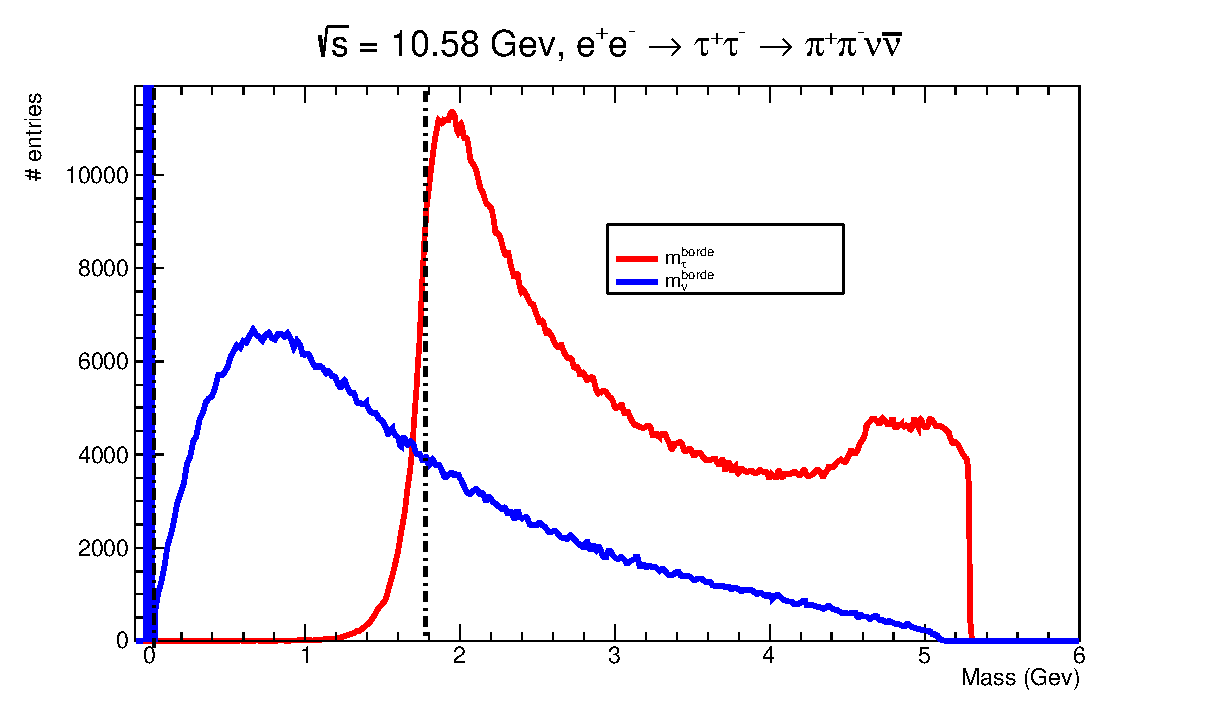
\includegraphics[scale=.6]{Images/m_edge.eps}
    \caption{\small Distribuciones para las variables de ``borde'' (\(m_{\tau}^{borde}\) y \(m_{\nu}^{borde}\)) para \(e^+e^-\rightarrow\tau^+\tau^-\rightarrow\pi^+\pi^-\nu\bar{\nu}\). Las líneas punteadas denotan la masa verdadera \(m_{\tau}\) y \(m_{\nu}\), que para nuestro caso es el valor que se utilizará para la generación (1777.0 MeV).}
    \label{fig:masas}
\end{figure}
\newpage
Tomando las ecuaciones \ref{39} y \ref{41}, una energía CM de 10.5794 \(GeV\)( justo la energía umbral de la resonancia \(\Upsilon(4S)\)), además teniendo encuentra nuestra consideración como límite físico para \(m_X\) de \(\sqrt{s}/2\) y por medio del software ROOT se construyeron las distribuciones (figura \ref{fig:masas}) para el proceso  \(e^+e^-\rightarrow\tau^+\tau^-\rightarrow\pi^+\pi^-\nu\bar{\nu}\).

\subsubsection{Variables ``\texorpdfstring{$M_{min}$}{TEXT}'' y ``\texorpdfstring{$M_{max}$}{TEXT}''}
Para esta parte del proceso, vamos a encontrar un par de variables, reduciendo el potencial del método de estados finales semi-invisibles para el caso en que tanto en señal como en tag tendremos iguales decaimientos 1x1 prong, este proceso es basado en el paper \cite{PhysRevD.102.115001}. 

Usando la ecuación \ref{24} vamos a reproducir otro método para encontrar la masa del leptón tau. Por practicidad, vamos a considerar \(\mu_{1} = \mu_{\nu_{\tau}}\) y \(\mu_{X}=\mu_{\tau}\). Asumiendo \(m_{\nu_{\tau}}=0\), la ecuación \ref{24} se reduce a
\begin{equation}
    A_0(\mu_{\tau}^2)^2+B_0(\mu_{\tau}^2)+D_0\leq0.
\end{equation}
Lo que nos lleva de nuevo a la ecuación \ref{40}, con lo cual
\begin{equation}
    (\mu_{\tau}^2)^2=\pm\frac{\sqrt{B_0^2-4A_0D_0}}{2A_0}-\frac{B_0}{2A_0},
\end{equation}
esto se puede ver como
\begin{equation}
    \left(\mu_{\tau}^{min}\right)^2\leq(\mu_{\tau})^2\leq\left(\mu_{\tau}^{max}\right)^2,
\end{equation}
ya que \(m_{\tau}=\mu_{\tau}\sqrt{s}\), entonces
\begin{equation}
    M_{min}^2\leq m_{\tau}^2 \leq M_{max}^2,
\end{equation}
donde
\begin{eqnarray}
    M_{min}^2&=&\left(\sqrt{s}\right)^2\left(\frac{-B_0-\sqrt{B_0^2-4A_0D_0}}{2A_0}\right),\\
    M_{max}^2&=&\left(\sqrt{s}\right)^2\left(\frac{-B_0+\sqrt{B_0^2-4A_0D_0}}{2A_0}\right).
\end{eqnarray}

Tomando las expresiones anteriores se construyen las distribuciones para las variables \(M_{min}\) y \(M_{max}\) (figura \ref{fig:MminMmaxDistri}), las cuales serán también métodos a probar y que se compararán con el método de ``borde'' para la estimación de la masa del leptón tau.
\begin{figure}[h]
    \centering
    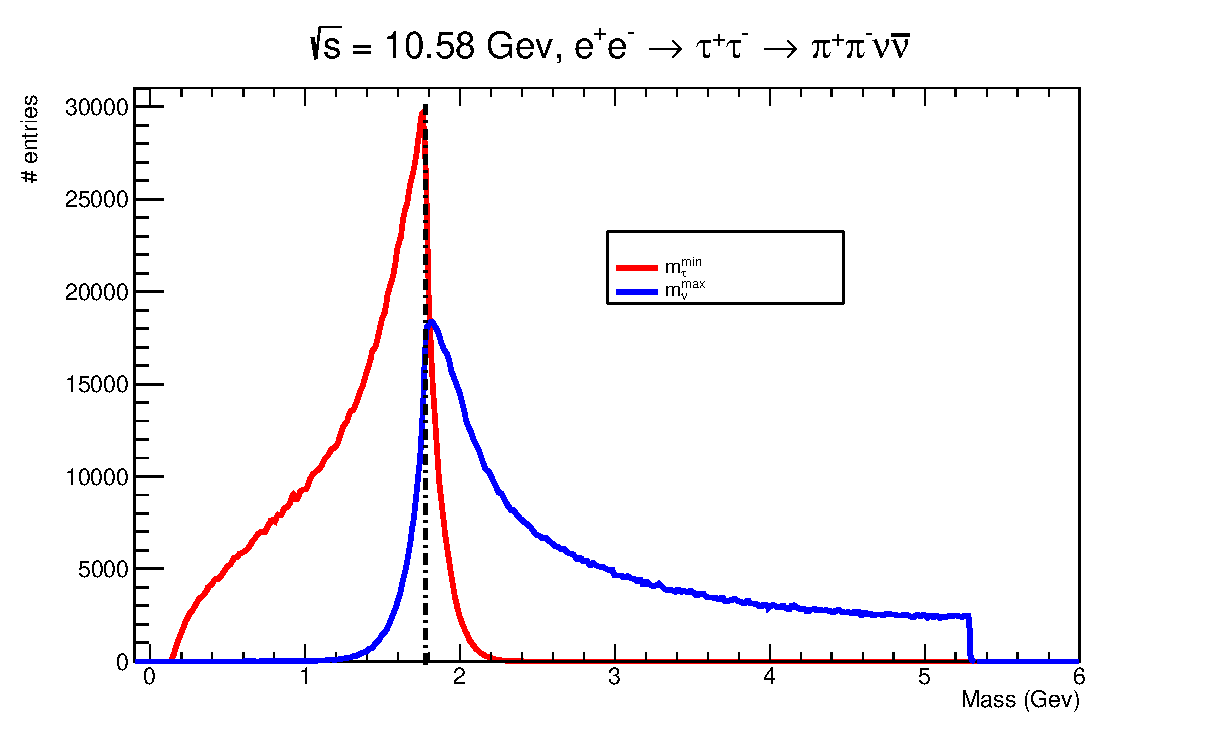
\includegraphics[scale=.6]{Images/m_min_plot.eps}
    \caption{\small{Distribuciones de las variables \(M_{min}\) (rojo) y \(M_{max}\) (azul). La línea punteada es la masa verdadera \(m_{\tau}\).}}
    \label{fig:MminMmaxDistri}
\end{figure}

Como se puede observar en las distribuciones \ref{fig:masas} y \ref{fig:MminMmaxDistri}, la masa que buscamos se relaciona con puntos donde dichas distribuciones tienen una subida pronunciada, son estos puntos los que estimaremos, para esto utilizaremos una función que contiene un parámetro que denominamos estimador.

\subsubsection{Estimador} 
Para ajustar las distribuciones se ha decidido implementar unas funciones de tipo sigmoide, la que mejor se adaptó al ajuste fue la función error complementaria para el caso de la variable \(M_{min}\) y tipo error para las variables \(M_{borde}\) y \(M_{max}\). Por la forma de las distribiciones se decidió multiplicarla por un polinomio para que reproduzca la caída luego de la subida prominente y sumarle un polinomio de segundo orden para ajustar la suave ``cola'' que es común en las tres distribuciones, las funciones de ajuste elegidas son las siguientes
\begin{equation}
    F_1(M_{\tau})=(P_3+P_4M_{\tau}+P_6M_{\tau}^2+P_7M_{\tau}^3)erfc\left(\frac{M_{\tau}-P_1}{P_2}\right)+P_8M_{\tau}^2+P_5M_{\tau}+1, \label{52}
\end{equation}
\begin{equation}
    F_2(M_{\tau})=(P_3+P_4M_{\tau}+P_6M_{\tau}^2+P_7M_{\tau}^3)erf\left(\frac{M_{\tau}-P_1}{P_2}\right)+P_8M_{\tau}^2+P_5M_{\tau}+1, \label{53}
\end{equation}
donde \(P_1\) es el estimador para la masa del leptón tau. Debido a que se busca una función que reproduzca adecuadamente a los datos en una zona de interés, la parametrización es completamente empírica y no un proceso analítico. Por otro lado, el estimador no será exactamente la masa del tau, pero se asumirá que este estará recorrido del valor real, así que se tendrá que corregir el valor del estimador para la función seleccionada en datos simulados, para esto empleamos una muestra oficial de Monte Carlo (MC13a) para la producción de pares de taus, para los cuales sabemos la masa de generación (1777 MeV).

\section{Criterio de selección de datos}
Para la selección de datos se usaron criterios tanto en las trayectorias de las partículas cargadas, como en los fotones, y se utilizaron los siguientes parámetros
\begin{table}[h!]
\centering
 \begin{tabular}{||c | c||} 
 \hline
 Criterio de trayectorias & Criterio para fotones  \\ [0.5ex] 
 \hline\hline
 \(p_t\)>0.1(GeV) & E> 0.2 (GeV)\\ 
 \hline
 -0.8660< cosTheta< 0.9563 & -0.8660< cosTheta< 0.9563  \\
 \hline
 -3.0< dz< 3.0 & clusterNHits> 1.5  \\
 \hline
 dr< 1.0 & 0.115 < M < 0.152  \\
 \hline
 \end{tabular}
 \caption{\small{Criterio de selección para las trayectorias de partículas cargadas y para fotones}}\label{table:crite}
\end{table}

De la tabla \ref{table:crite}, \(p_t\) es el el momento transversal de la partícula cargada, E sería la energía del fotón, \(cosTheta\) es el coseno del ángulo que comprende el detector (aceptancia del detector), \(dz\) es la distancia de la reconstrucción de la trayectoria respecto al IP sobre el eje z, \(dr\) es la distancia de la misma en la coordenada radial. Ambos valores, \(dz\) y \(dr\) están expresados en \(cm\). Por otro lado, el parámetro \(clusterNHits\) hace referencia el número de cristales activados en el ECL para reconstruir un fotón. 0.115 < M < 0.152 es el criterio para la reconstrucción de \(\pi^0\)'s. 

La selección de eventos requirió que se hiciera un filtrado haciendo algunos cortes en ciertas variables, para ello se utilizaron los siguientes \begin{table}[h!]
\centering
 \begin{tabular}{||c||} 
 \hline
 Criterio de selección de eventos \\ [0.5ex] 
 \hline\hline
 nGoodTracks = 2 \\ 
 \hline
 Thrust<0.99 \\
 \hline
 0<EoverP<0.8 \\
 \hline
 N(\(\pi^0\))=0\\
 \hline
 N(\(\gamma\))\leq1\\
 \hline
 \end{tabular}
 \caption{\small{Criterio de selección de eventos}}\label{table:crite}
\end{table}

\(nGoodTracks\) es el número de buenas partículas cargadas, para nuestro caso usamos dos, y así reproducir la topología que nos interesa. \(Thrust\) es una variable que se define por medio del vector unitario \(\hat{u}_{thrust}\) perpendicular a la línea que separa la señal y  (figura \ref{fig:MminTopo}), el valor del \(Thrust\) se define como \(V_{thrust}\equiv\sum_{i}\frac{|\mathbf{p}_i^{cm} \cdot \hat{n}_{thrust}|}{\sum_{i}|\mathbf{p}_{j}^{cm}|}\), de manera que dicho valor sea el máximo,  Con el vector \(\hat{n}_{thrust}\) y el valor del thrust se separan los decaimientos en dos hemisferios. La variable EoverP que es la razón entre la energía depositada en el calorímetro y el momento de partículas cargadas, se exige 0<\(EoverP\)<0.8 para garantizar una mayor cantidad de piones presentes en los tracks (esta variable se usó en el proceso de reconstrucción en la variable \(pionIDcuts\)). \(N(\pi^0)\) es el número de piones neutros y \(N(\gamma)\) es el número de fotones.
\begin{figure}[h]
    \centering
    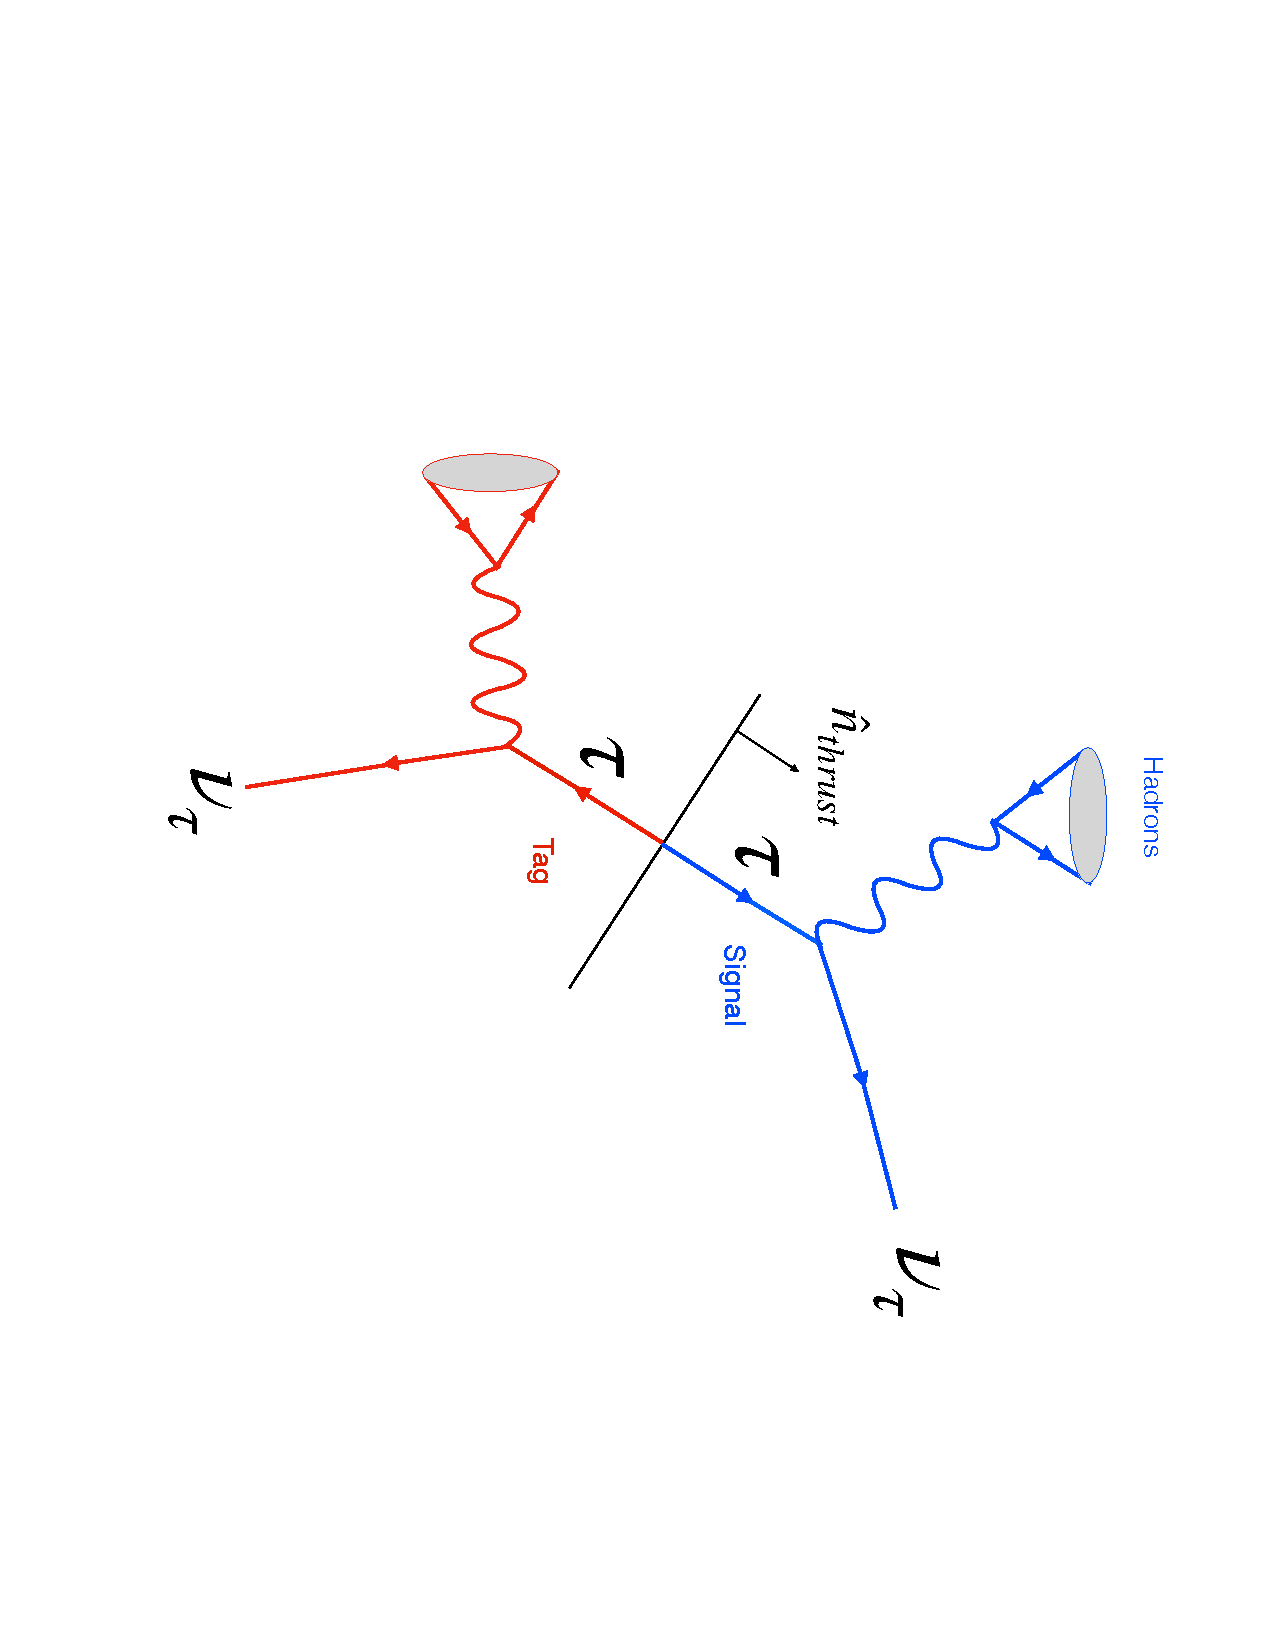
\includegraphics[scale=.05]{Images/Diagram1x1.jpg}
    \caption{\small{Esquema señal-tag en topología 1x1 prong en decaimiento del tau. Se muestra la dirección del vector \(\hat{n}_{thrust}\) que separa la señal del tag.}}
    \label{fig:MminTopo}
\end{figure}

Con los requerimientos anteriores, tanto de trayectorias, como en fotones y en selección de eventos se reconstruyeron los pares de taus que cumplen dichos requisitos, decayendo tanto tag como señal en 1-prong, para nuestro caso, en un pión cargado y un neutrino del tau. Con esta información se logra hacer la reconstrucción del par de taus (taupair).

\section{Database}

Se utilizaron como datos, los generados mediante método Monte Carlo en la campaña oficial de Belle II MC13a. Los datos fueron tratados como si provinieran directamente del detector, es decir, sobre ellos se aplicaron los cortes de selección de eventos, a esto se le conoce como ``skim''. La muestra de MC usada es equivalente a una luminosidad de 100 \(fb^{-1}\) (Cantidad de datos equiparable con los datos que hasta hace poco se habían recolectado en Belle II, cifra superada en junio del 2021, hasta el momento se han recolectado 200 \(fb^{-1}\)), las muestras de MC usadas se pueden separar en dos, Generic (Genérica) y Lowmulti (Baja multiplicidad) como se observa en la tabla \ref{table:skim}. En la versión release-04-00-03 del software basf2 se reconstruyó el decaimiento de interés, usando Tauola que proporciona todos los posibles decaimientos del leptón tau. Las muestras se generan en la colaboración para una masa de 1777 \(MeV\), siendo para este estudio considerada la masa verdadera.
\begin{table}[h!]
\centering
 \begin{tabular}{|| p{3cm} | p{3cm} | p{3.5cm} ||} 
 \hline
 Etiqueta de producción & Tipo de evento & Luminosidad \\ [0.5ex] 
 \hline\hline
 MC13a  & mixed & 100 \(fb^{-1}\), \\
 (Generic)& &\\
 & charged &\\
 & & correspondiente a\\
 & uubar & mixed: 51 M\\
 & & charged: 54 M\\
 & ddbar & uubar: 160.5 M\\ 
 & & ddbar: 40.1 M\\
 & ccbar & ssbar: 38.3 M\\
 & & ccbar: 132.9 M\\
 & ssbar & taupair: 91.9 M\\
 & &\\
 & taupair &\\
 \hline
 MC13a  & eeee & 100 \(fb^{-1}\) \\
 (Lowmulti)& &\\
 & mumu &\\
 & & \\
 & eemumu &\\
 &\hline&\hline \\
 & ee & 10 \(fb^{-1}\)\\
 \hline
 \end{tabular}
 \caption{\small{Muestras de la campaña MC13a, Generic y Lowmulti con su correspondiente luminosidad}}\label{table:skim}
\end{table}
 Tendremos como señal el proceso de decaimiento \(\tau\rightarrow\pi\nu_{\tau}\), este se encuentra dentro de la muestra "taupair", dicha muestra se filtró inicialmente con los cortes de selección, luego con los criterios de selección de eventos y por último usando la variabe ``\(MCMode\)'', esta permite seleccionar el decaimiento que nos compete con un indicador como se muestra en la figura \ref{fig:TauDecay} , donde el modo de decaimiento 1x1-prong usado es el número 3. Ya seleccionando la señal se creó el histograma de la distribución para cada una de las variables que se estudiaron.
\begin{figure}[h]
    \centering
    \includegraphics[scale=.8]{Images/TauDecays.png}
    \caption{\small{Marcadores para los distintos decaimientos del tau presentes en TauolaBelle, la variable de identificación de estos canales es denominada \textit{MCMode}}}.
    \label{fig:TauDecay}
\end{figure}

\subsection{Estimador para \texorpdfstring{$M_{borde}$}{TEXT}}
Los demás procesos que no sean el decaimiento que denominamos como señal son considerados como ruido. Para este trabajo se consideran procesos de baja multiplicidad (\(ee,ee\mu\mu,\mu\mu,eeee\)), \(q\bar{q}\) (\(q = u,d,s,c\)), \(B\bar{B}\) y todos los procesos posibles en decaimientos del leptón tau (figura \ref{fig:TauDecay}), de estos últimos se hace la distinción entre señal y ruido. La señal es el proceso \(\tau\rightarrow\pi\nu\), los demás decaimientos del tau serán considerados como ruido y la denominaremos como ``\(\tau\)BG''. Al agregar todas las muestras anteriores a una sola distribución se reproduce la distribución que se obtendría con datos reales de Belle II. Para obtener la señal se debe separar señal de ruido, para esto se decide usar un método de Maching Learning, como lo son los BDT (\textit{Boosting Decision Trees}), implementado en ROOT por medio de un ambiente para el procesamiento y evaluación de clasificación multivariada como lo es TMVA (\textit{Toolkit for Multivariate Data Analysis}) \cite{Hocker:2007ht}.

\subsubsection{BDT}

Por medio de TMVA y usando catorce variables cinemáticas de evento y dos de identificación de partículas se hizo el entrenamiento para el BDT. Las variables usadas fueron las siguientes.


\begin{itemize}
    \item \textit{track1\_cosToThrustOfEvent}:  coseno del ángulo entre la partícula cargada y el eje de thrust del evento.
    \item 
    \textit{track1\_clusterE}: energía del clúster ECL corregida por fugas y ruido.
    \item 
    \textit{visibleEnergyOfEventCMS}: energía visible en el marco de referencia CM.
    \item
    \textit{missingMomentumOfEventCMS}: magnitud del momento perdido en el marco de referencia CM
    \item
    \textit{missingMomentumOfEventCMS\_theta}: ángulo \(\theta\) del momento perdido en el CM
    \item
    \textit{missingMass2OfEven}: masa perdida al cuadrado
    \item
    \textit{track1\_EoverP}: EoverP de la partícula cargada del track 1
    \item
    \textit{track1\_pt}: momento total del track 1
    \item
    \textit{track1\_pionID}: pionID para el track 1
\end{itemize}

Así como las variables correspondientes a la otra partícula cargada del decaimiento que se denomina ``track2''.

Uno de los resultados del BDT fue que las variables que más separación entre ruido y señal aportaron fueron las de \(pionID\). El TMVA crea las distribuciones de clasificación (figura \ref{fig:bdtFom}), con ayuda de dicha distribución se debe seleccionar el mejor corte en esta variable nueva (BDT), y así garantizar una eficiencia óptima en la separación ruido-señal, para encontrar el mejor valor de BDT se usó la figura de mérito
\begin{equation}
    FOM=2\left(\sqrt{N_{sig}+N_{bkg}}-\sqrt{N_{bkg}}\right)\label{fom},
\end{equation}
obteniéndose un valor para el BDT de alrededor de 0.2, nótese que dicho valor es el punto donde la FOM tiene un máximo. Se elige para el método \(m^{borde}_{\tau}\) un valor del BDT de 0.2. Las muestras se han dividido en tres partes. La primera para realizar el entrenamiento del TMVA y crear los BDT's, la segunda será para encontrar el estimador y el sesgo de los diferentes métodos y la tercera se usará como ``datos reales'' para el análisis final y estimación de la masa del leptón tau en cada método.
\begin{figure}%
    \centering
    \subfloat[\centering  ]{{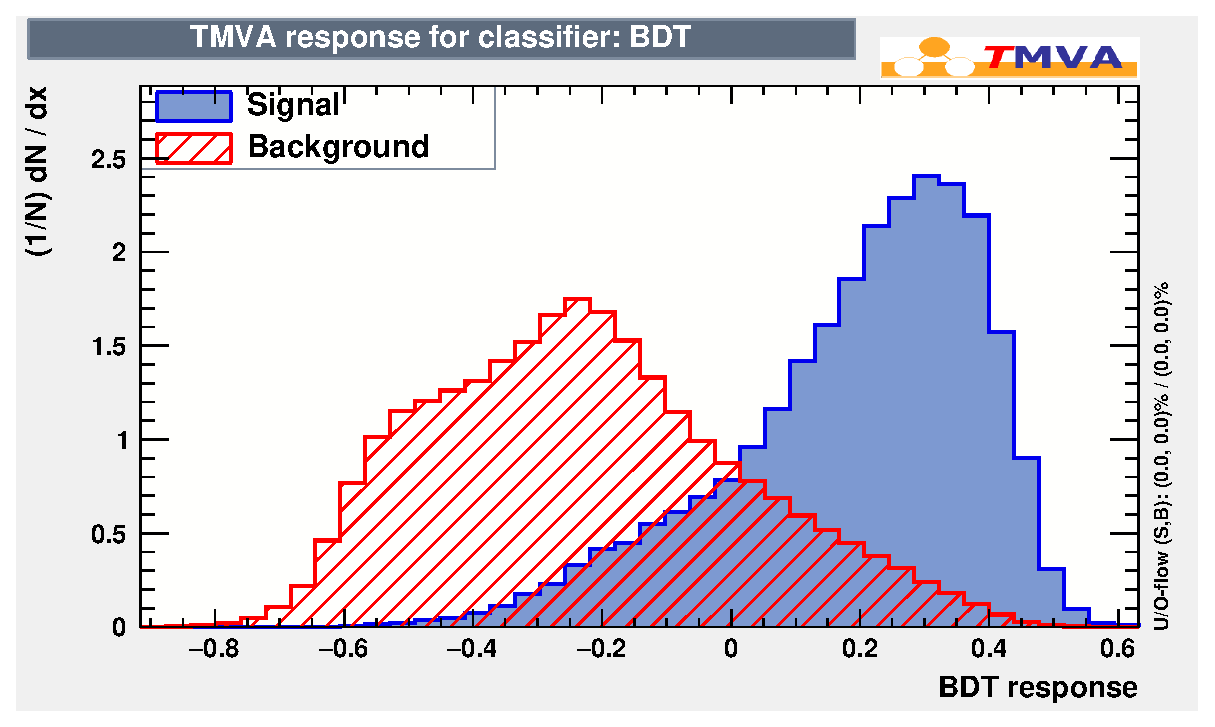
\includegraphics[width=7.5cm]{Images/bdt_bg_sig.eps} }}%
    \qquad
    \subfloat[\centering  ]{{\includegraphics[width=7.5cm]{Images/FOM.png} }}%
    \caption{(a) Distribución de respuesta del BDT y clasificada como señal y ruido. (b) FOM}
    \label{fig:bdtFom}%
\end{figure}
Inicialmente, se grafica la distribución de la variable \(m^{borde}_{\tau}\) sólo para señal y se muestra la distibución completa y un zoom en la región de ajuste en la figura \ref{fig:mEdgeDistri}, esto con propósito de tener bien definida la señal y para realizar el ajuste más óptimo. 

De la figura \ref{fig:ajusteMedge}, en la región de ajuste se observan dos grandes componentes, una es la principal que se refiere a la señal y la otra es el ruido de fondo \(\tau\)BG. Lo anterior luego de hacer el corte en BDT, se deben ajustar ambas componentes y unirlas en una sola para encontrar el estimador para la masa del leptón tau. Se elije usar para la componente de \(\tau\)BG una función de ajuste o función de distribución de probabilidad (PDF) de tipo lineal de la forma
\begin{equation}
    F_3(M_{\tau})=A_1+A_2M_{\tau}, \label{55}
\end{equation}
con la ayuda de la PDF \ref{53} se ajustó la señal y el ruido se ajustó con \ref{55}, luego se debían unir ambos ajustes, es decir ``sumar'' las PDF's, para ello se usó una suma paramétrica de la forma
\begin{equation}
    F_{4}=fS_{PDF}+(1-f)B_{PDF},
\end{equation}
donde \(S_{PDF}\) es la PDF para la señal, \(B_{PDF}\) la PDF para el ruido y \(f\) es un coeficiente menor que 1, es decir, es una constante sujeta a las condiciones de normalización.


Para una muestra de pares tau se realizó la medición de la masa y se compara el estimador con el valor de la masa de generación \(m_{\tau}=1777.00\) MeV. Para el caso de la variable \(M_{borde}\) en la región de ajuste y utilizando la adición de PDF's se obtuvo un valor para el estimador \(P1=1765.80\pm6.0\) MeV (figura \ref{fig:ajusteMedge} (a)), la diferencia en la masa es de \(\Delta_{m}=11.2\) MeV. Con este valor de bias se corrige el valor obtenido con la muestra restante, la de datos reales (figura \ref{fig:ajusteMedge} (b)), corregimos la estimación de la masa para los datos reales, obtenemos un valor para la masa del tau de \(m_{\tau} = 1772.40\pm 7.38\) MeV. Para el valor final en las incertidumbres se decidió combinarla y para ello se usó la suma en cuadraturas. 

\begin{figure}[h]
  %\setcapwidth{0.6\textwidth}
  \checkoddpage
  \edef\side{\ifoddpage r\else l\fi}%
  \makebox[\textwidth][\side]{%
    \begin{minipage}[t]{0.58\textwidth}
      \centering
    \subfloat[\centering  ]{{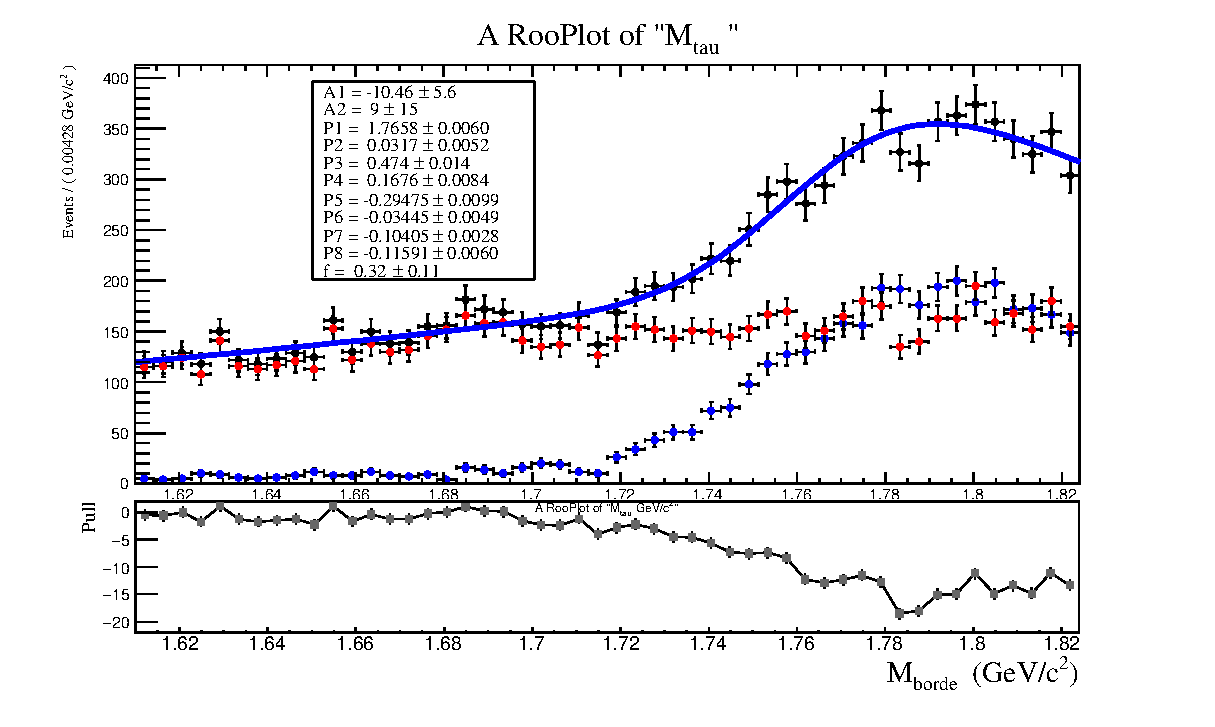
\includegraphics[width=\textwidth]{Images/m_borde_bkg_sig.eps} }}
      %\caption{Caption 1}
    \end{minipage}%
    \hfill
    \begin{minipage}[t]{0.58\textwidth}
      \centering
    \subfloat[\centering  ]{{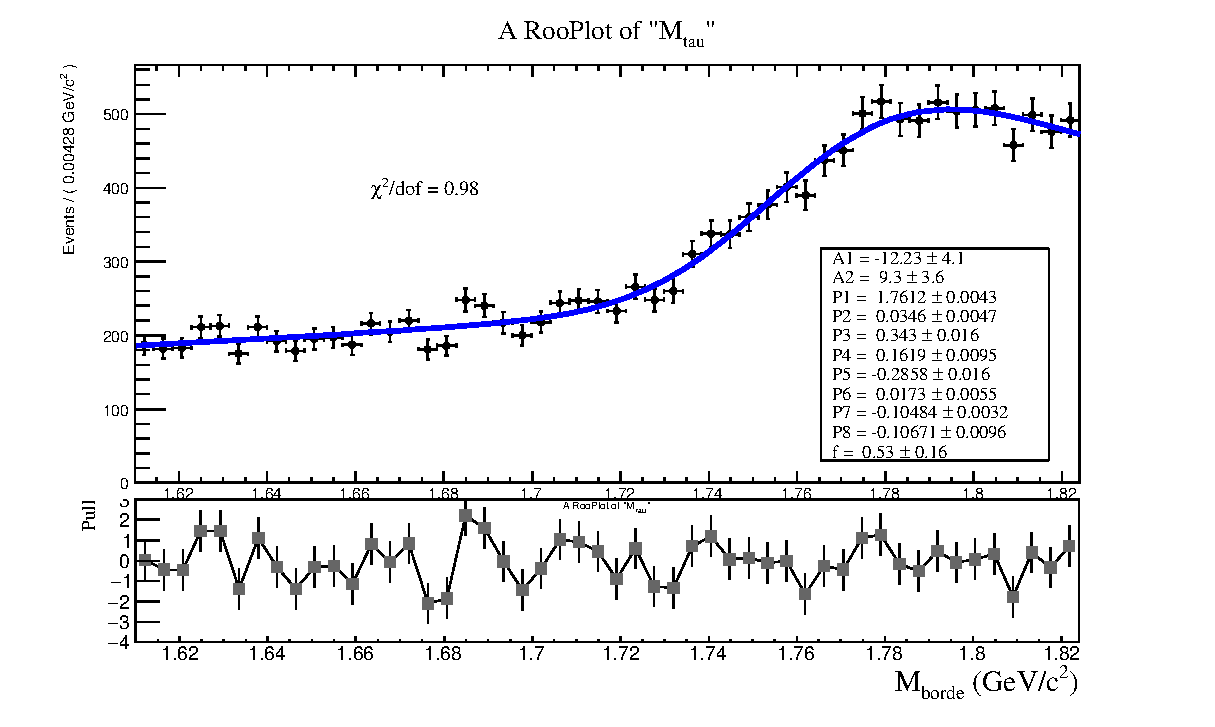
\includegraphics[width=\textwidth]{Images/m_borde_real.eps} }}
      %\caption{Caption 2}
    \end{minipage}%
  }%
  \caption{\small{(a) Ajuste \(M_{borde}\) para ruido y señal. En rojo \(\tau BG\), en azul \(\tau \rightarrow \pi\nu \) y en negro la suma de señal más ruido. Valor para el estimador de la masa de \(1765.8\pm5.2\) MeV.  (b) Ajuste de la distribución de la variable \(M_{borde}\) para datos ``reales'' con un valor para el estimador de la masa de \(1761.2\pm4.3\) MeV.}}
  \label{fig:ajusteMedge}
\end{figure}

\newpage
\subsection{Estimador para \texorpdfstring{$M_{min}$}{TEXT}}



Para el caso de la variable \(M_{min}\) se muestra la distribución completa de sólo señal y en la región de ajuste en la figura \ref{fig:mMinDistri}. Usando el corte BDT>0.2, se separa en esta variable señal de ruido de una forma más prolija, las contribuciones de ruido se pueden ver en las figuras del apéndice B. En la zona de ajuste se observa que el ruido \(\tau BG\) contribuye menos que en el caso anterior, pero se decide de igual forma usar la PDF para el ruido (\ref{55}) y para la señal la función error complementaria (\ref{52}), gráficamente este proceso se puede ver en la figura \ref{fig:ajusteMmin} (a).

Se obtiene un valor para el estimador de \(P1=1777.70\pm 0.16\) MeV, una diferencia respecto al valor real de \(\Delta_{m}=-0.70\) MeV. Ya considerando la muestra real (figura \ref{fig:ajusteMmin} (b)) y con el valor de la diferencia corregimos la estimación de la masa y en datos reales  se obtiene un valor para la masa del leptón tau de \(m_{\tau} = 1777.06 \pm 0.47\) MeV.
\begin{figure}[h]
  %\setcapwidth{0.6\textwidth}
  \checkoddpage
  \edef\side{\ifoddpage l\else r\fi}%
  \makebox[\textwidth][\side]{%
    \begin{minipage}[t]{0.57\textwidth}
      \centering
    \subfloat[\centering  ]{{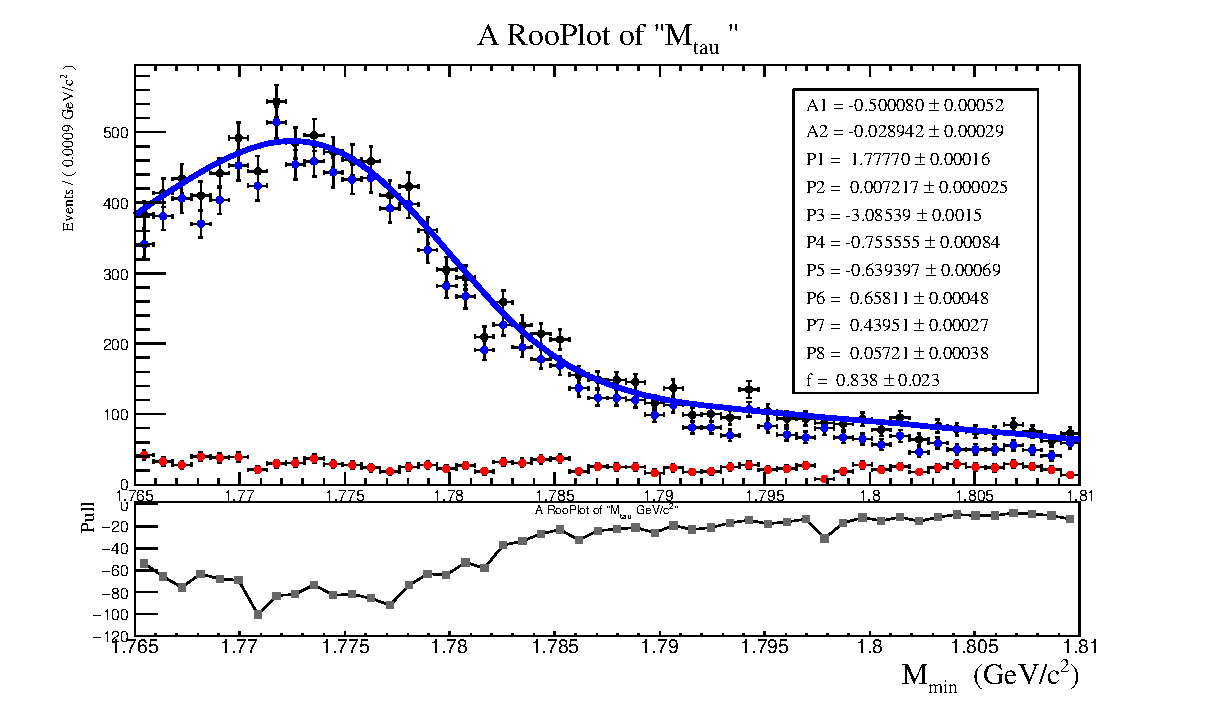
\includegraphics[width=\textwidth]{Images/m_min_bkg_sig.eps} }}
      %\caption{Caption 1}
    \end{minipage}%
    \hfill
    \begin{minipage}[t]{0.57\textwidth}
      \centering
    \subfloat[\centering  ]{{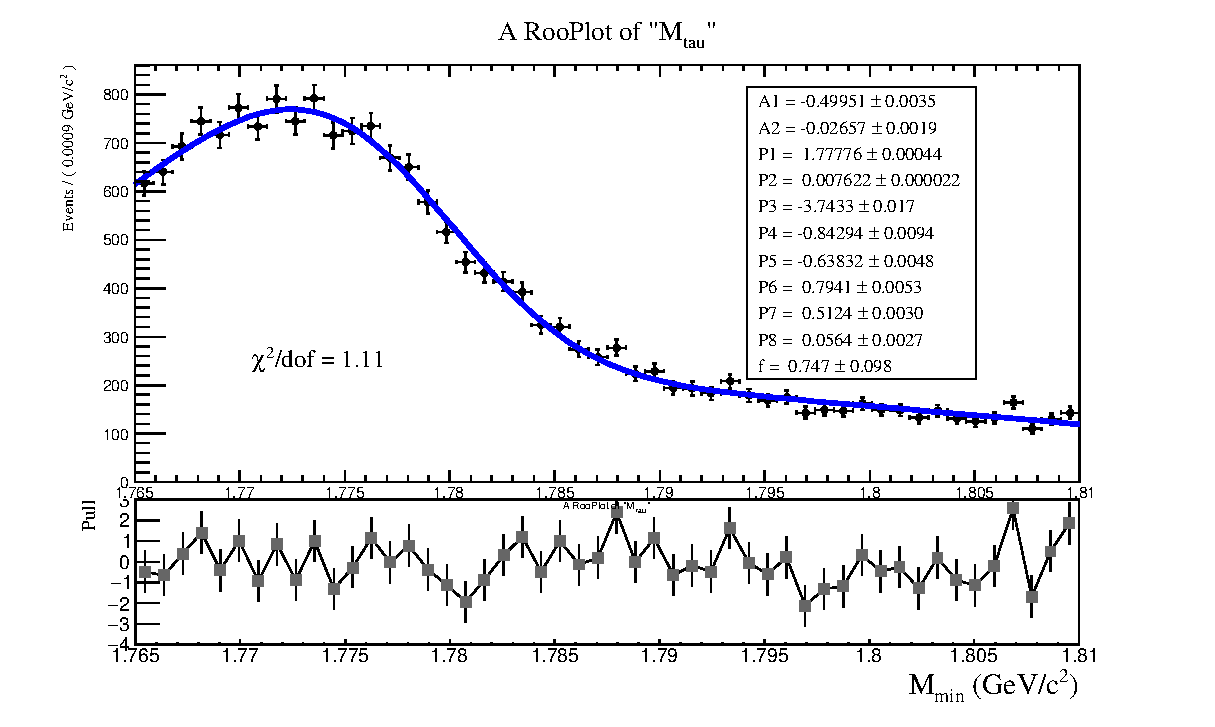
\includegraphics[width=\textwidth]{Images/m_min_real.eps} }}
      %\caption{Caption 2}
    \end{minipage}%
  }%
  \caption{\small{(a) Ajuste de \(M_{min}\) para ruido y señal. En rojo \(\tau BG\), en azul, \(\tau \rightarrow \pi\nu \) y en negro la suma de señal más ruido. Valor para el estimador de la masa de \(1777.70\pm0.16\) MeV.  (b) Ajuste de la distribución \(M_{min}\) en datos reales con un valor para el estimador de la masa de \(1777.76\pm0.44\) MeV.}}
  \label{fig:ajusteMmin}
\end{figure}


\newpage
\subsection{Estimador para \texorpdfstring{$M_{max}$}{TEXT}}

Siguiendo el mismo proceso para el último método, la variable \(M_{max}\) sólo considerando señal, se muestra la distribución completa junto con el zoom en la región de ajuste en el apéndice C. En este caso se logra obtener un valor para el estimador de masa de \(P1=1775.16\pm0.14\) MeV (figura \ref{fig:ajusteMmax} (a)) para una diferencia en la masa de \(\Delta_{m}=1.84\) MeV. Corrigiendo entonces con este bias al valor obtenido en el ajuste a los datos reales se obtiene un valor para la masa de \(m_{\tau}=1781.44\pm0.38\) MeV.
\begin{figure}[h]
  %\setcapwidth{0.6\textwidth}
  \checkoddpage
  \edef\side{\ifoddpage r\else l\fi}%
  \makebox[\textwidth][\side]{%
    \begin{minipage}[t]{0.57\textwidth}
      \centering
    \subfloat[\centering  ]{{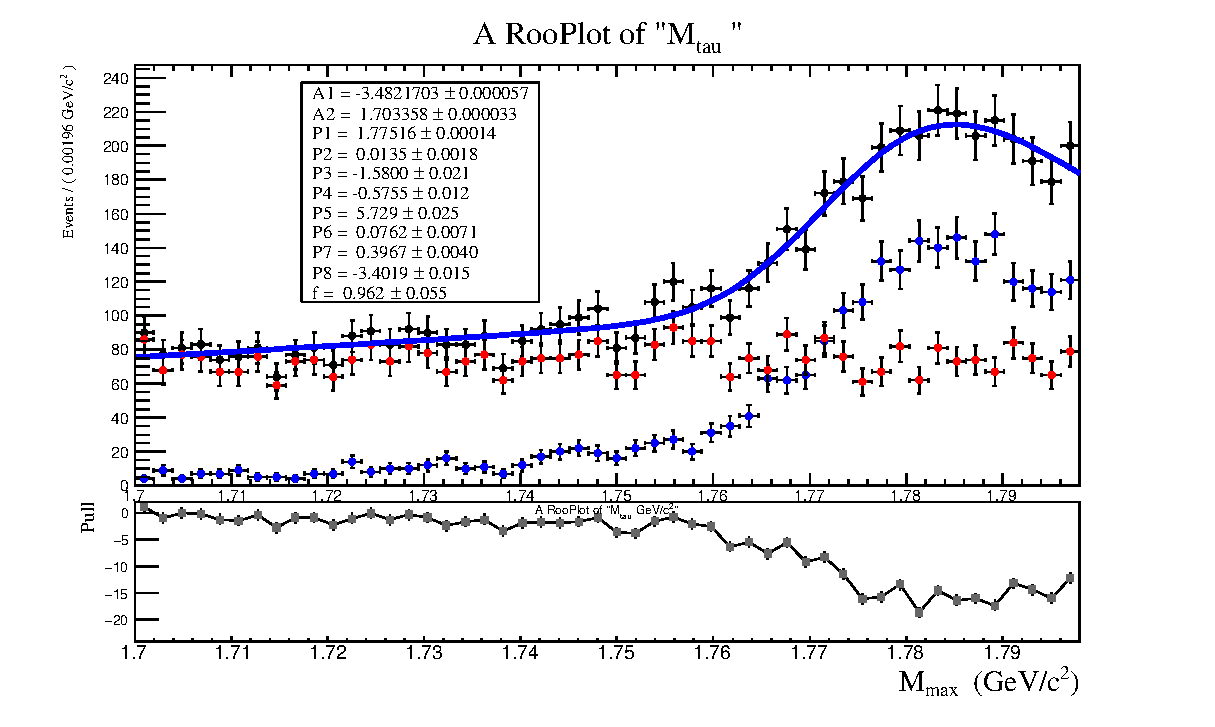
\includegraphics[width=\textwidth]{Images/m_max_bkg_sig.eps} }}
      %\caption{Caption 1}
    \end{minipage}%
    \hfill
    \begin{minipage}[t]{0.57\textwidth}
      \centering
    \subfloat[\centering  ]{{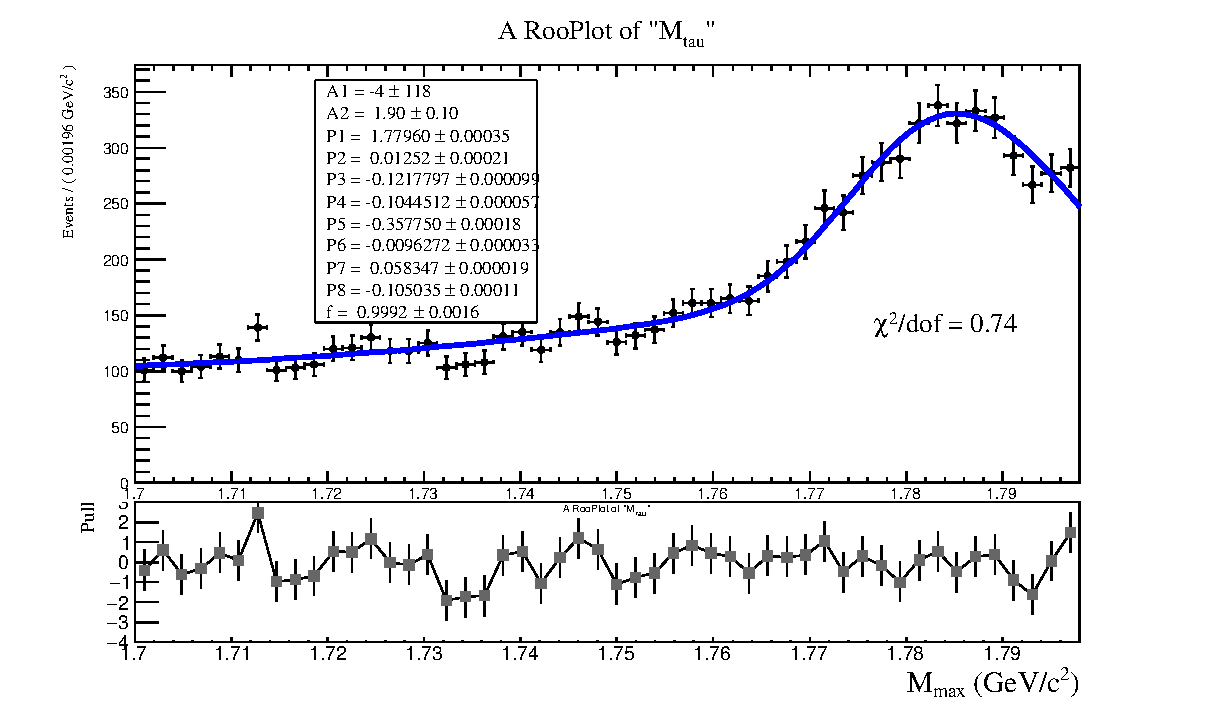
\includegraphics[width=\textwidth]{Images/m_max_real.eps} }}
      %\caption{Caption 2}
    \end{minipage}%
  }%
  \caption{\small{(a) Ajuste de \(M_{max}\) para ruido y señal. En rojo \(\tau BG\), en azul, \(\tau \rightarrow \pi\nu \) y en negro la suma de señal más ruido. Valor para el estimador de la masa de \(1775.16\pm0.14\) MeV.  (b) Ajuste de la distribución de \(M_{max}\) en datos reales con un valor para el estimador de \(1779.60\pm0.35\) MeV.}}
  \label{fig:ajusteMmax}
\end{figure}
